\section{Results}\label{sec:results}

\subsection{Mechanism Combinations}\label{subsec:mechanism-combinations}
The absolute mean error as a percent of the total preference space by coordination
mechanism per voting mechanism is graphed in
\autoref{fig:vm-col-cm-hue-error-as-percent-of-space-abs-mean}.
% \vicki{Briefly describe how you define mean square error}
The absolute mean error as a percent of the total preference space
$\sigma_{\lvert M\% \rvert}$  is defined as
$
    \sigma_{\lvert M\% \rvert} =
    \frac{1}{n (\systemspace_{\max} - \systemspace_{\min})}
        \sum^{n}_{i = 1}{\lvert \epsilon_i  \rvert}
$,
where $n$ is the number of runs, $\systemspace_{\max}$ and $\systemspace_{\min}$ are
the maximum and minimum value in the preference space, respectively, and $\epsilon_i$
is the error of run $i$.
Error is defined as $\truthof{\text{proxy}}~-~\truthof{\text{baseline}}$, meaning the
output of the proxy run minus the output of the baseline (all agents voting).

From this plot, there are a few trends that are immediately identifiable.
First, error unsurprisingly increases as the number of inactive agents increases.
This is true with two notable exceptions: first, the Active Only/Median
mechanism combination has a somewhat sawtooth shape.
This is due to the Median mechanisms always choosing a specific agent's preference
instead of aggregating to some more preferential in-between value.

The second exception is that Mean coordination mechanism consistently dips when all but
one agent become delegators.
This is because we take the mean of the constituents and the proxy, then apply the
voting mechanism on the set of proxy-constituent votes.
Since there is only one agent, there is only one proxy-constituent vote and so the
result of the vote is the result of the coordination mechanism.
Essentially, the coordination mechanism replaces the voting mechanism.

We can also see the Mean and Median coordination mechanisms generally yield similar
amounts of error.
In particular, when either of these mechanisms is combined with the Mean voting
mechanism the results are very similar to when all agents are active and able to vote.

Notably, the Expert coordination mechanism works worse than the others as the number
of delegators reaches a significant portion of the population.
In particular, the Expert mechanism tracks nearly identically to Active Only when
using the Midrange voting mechanism.
Depending on the use case, this may or may not be beneficial.
If we are attempting to find the best result for all agents, this mechanism may yield
undesirable results.
However, if we are attempting to exploit the expert's experience, as described
by~\cite{Miller1969}, this error could actually be considered an improvement over
the original result.
This is because the experts were able to influence and change the vote, presumably
bringing it closer to what their expertise dictates.
Nevertheless, when the number of delegators is low, the Expert mechanism works
similarly to the other coordination mechanisms.

Importantly, it is clear that using proxy voting, regardless of the mechanisms used,
is better than losing information by not allowing inactive agents to vote in any way.

However, what if there was some penalty for the inactive agents?
Since they aren't participating as much, perhaps it would be fair that their voice is
not as strong.
We attempted the same experiments as above with different weights between a proxy and
their constituents.
Specifically, the proxies maintain their weight of 1, while their constituents have
their weight reduced to $\sfrac{1}{5}$ (0.2) of their original weight.
We choose $\sfrac{1}{5}$ because it still allows constituents to have some impact
while still having their influence significantly reduced.
The results of such a setup are shown
in~\autoref{fig:different-weight-vm-col-cm-hue-error-as-percent-of-space-abs-mean}.
\vicki{How do you define error in this case?  If you only give them a .2 vote, but compare to when they get a full vote, that seems meaningless.  We are giving them a .2 vote because their vote shouldn't count as much.  Can you compare the shift in results between the two methods?  I wouldn't call it an error, but the difference between the methods.  Better to have the comparison between the two on one graph rather than  having the reader compare two figures.}

These graphs immediately show there is an increase in error in all mechanisms. \vicki{which graphs are you referring to?  due to what?  unclear.}
This is due to the results of the vote becoming more biased towards the preferences
of the proxies.
Depending on the situation, this may be desirable.
Since the inactive agents are not participating they may not have as much information
and so their preference may not be as `up-to-date' as those who are actively
participating.
In situations where new information is constantly being introduced, such penalties
could be very valuable to ensure the most current information is being used.

\begin{landscape}
    \begin{figure}[p]
        \centering
        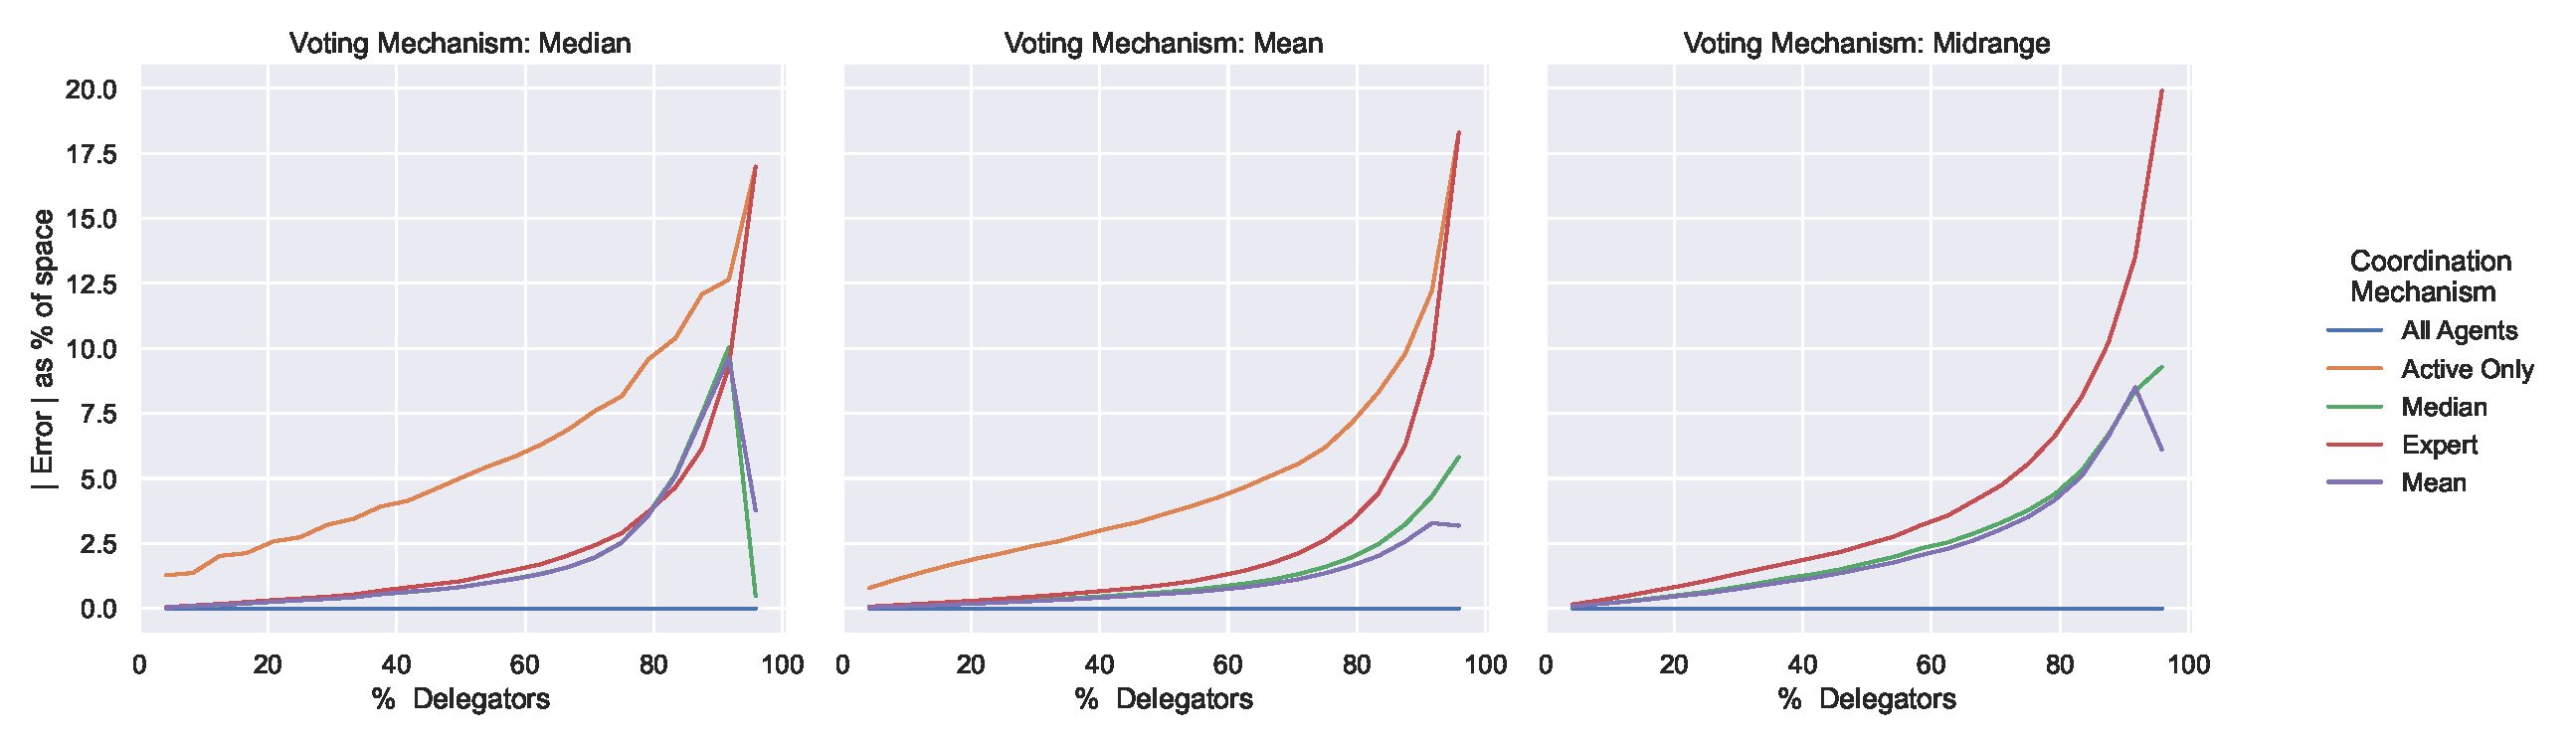
\includegraphics[scale=0.55]
        {content/chapter2/figures/vm_col_cm_hue_error_as_percent_of_space_abs_mean}
        \caption{
            The absolute mean error as a percent of the preference space by
            coordination mechanism per voting mechanism.
            `Error as a percent of the preference space' means the error divided by
            the total size of the preference space.
            Note All Agents represents when all agents are voting, meaning no proxy
            voting is used and all agents are present.
            Similarly, Active Only represents when proxy voting is not used and not
            all agents are present, and when proxies lose their constituents.
            Averaged over 1024 total runs.
            There are 24 total agents.
        }
        \label{fig:vm-col-cm-hue-error-as-percent-of-space-abs-mean}
    \end{figure}

    \begin{figure}[p]
        \centering
        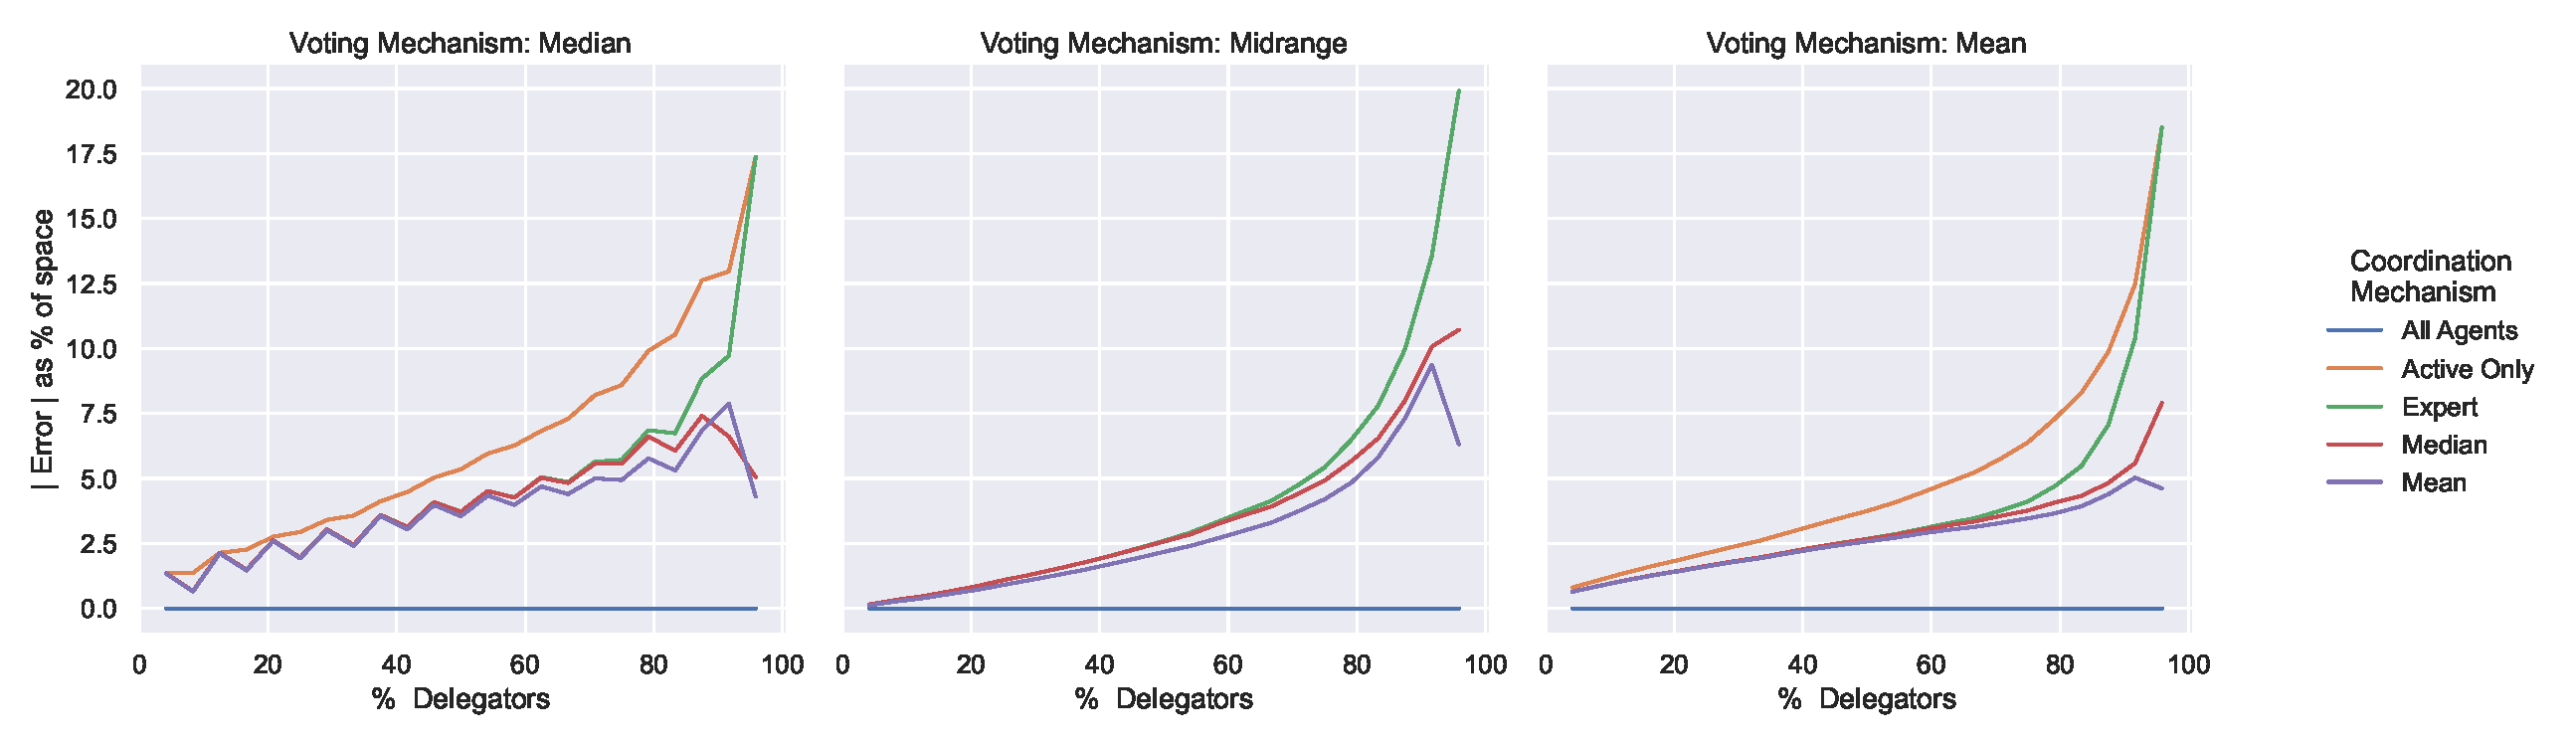
\includegraphics[scale=0.55]
        {content/chapter2/figures/different_weight/vm_col_cm_hue_error_as_percent_of_space_abs_mean}
        \caption{
            The absolute mean error as a percent of the preference space by
            coordination mechanism per voting mechanism.
            `Error as a percent of the preference space' means the error divided by
            the total size of the preference space.
            Note All Agents represents when all agents are voting, meaning no proxy
            voting is used and all agents are present.
            Similarly, Active Only represents when proxy voting is not used and not
            all agents are present, and when proxies lose their constituents.
            Averaged over 1024 total runs.
            There are 24 total agents.
            \\
            Proxies in this graph have a weight of 1, while their constituents have a
            weight of 0.2.
        }
        \label{fig:different-weight-vm-col-cm-hue-error-as-percent-of-space-abs-mean}
    \end{figure}
\end{landscape}

\subsection{By Distribution}\label{subsec:results-distribution}
\autoref{fig:distribution-error-as-percent-of-space-abs-mean} shows
the absolute error as a percent of the preference space by coordination mechanism for
each voting mechanism and preference distribution.
\autoref{fig:distribution-different-scale-error-as-percent-of-space-abs-mean} shows
the same graphs, but with a different scale for each plot to more easily see the shape.
Additionally, each graph is zoomed in for readability
in~\autoref{apx:error-by-dist-zoomed}.

\begin{figure}[p]
    \centering
    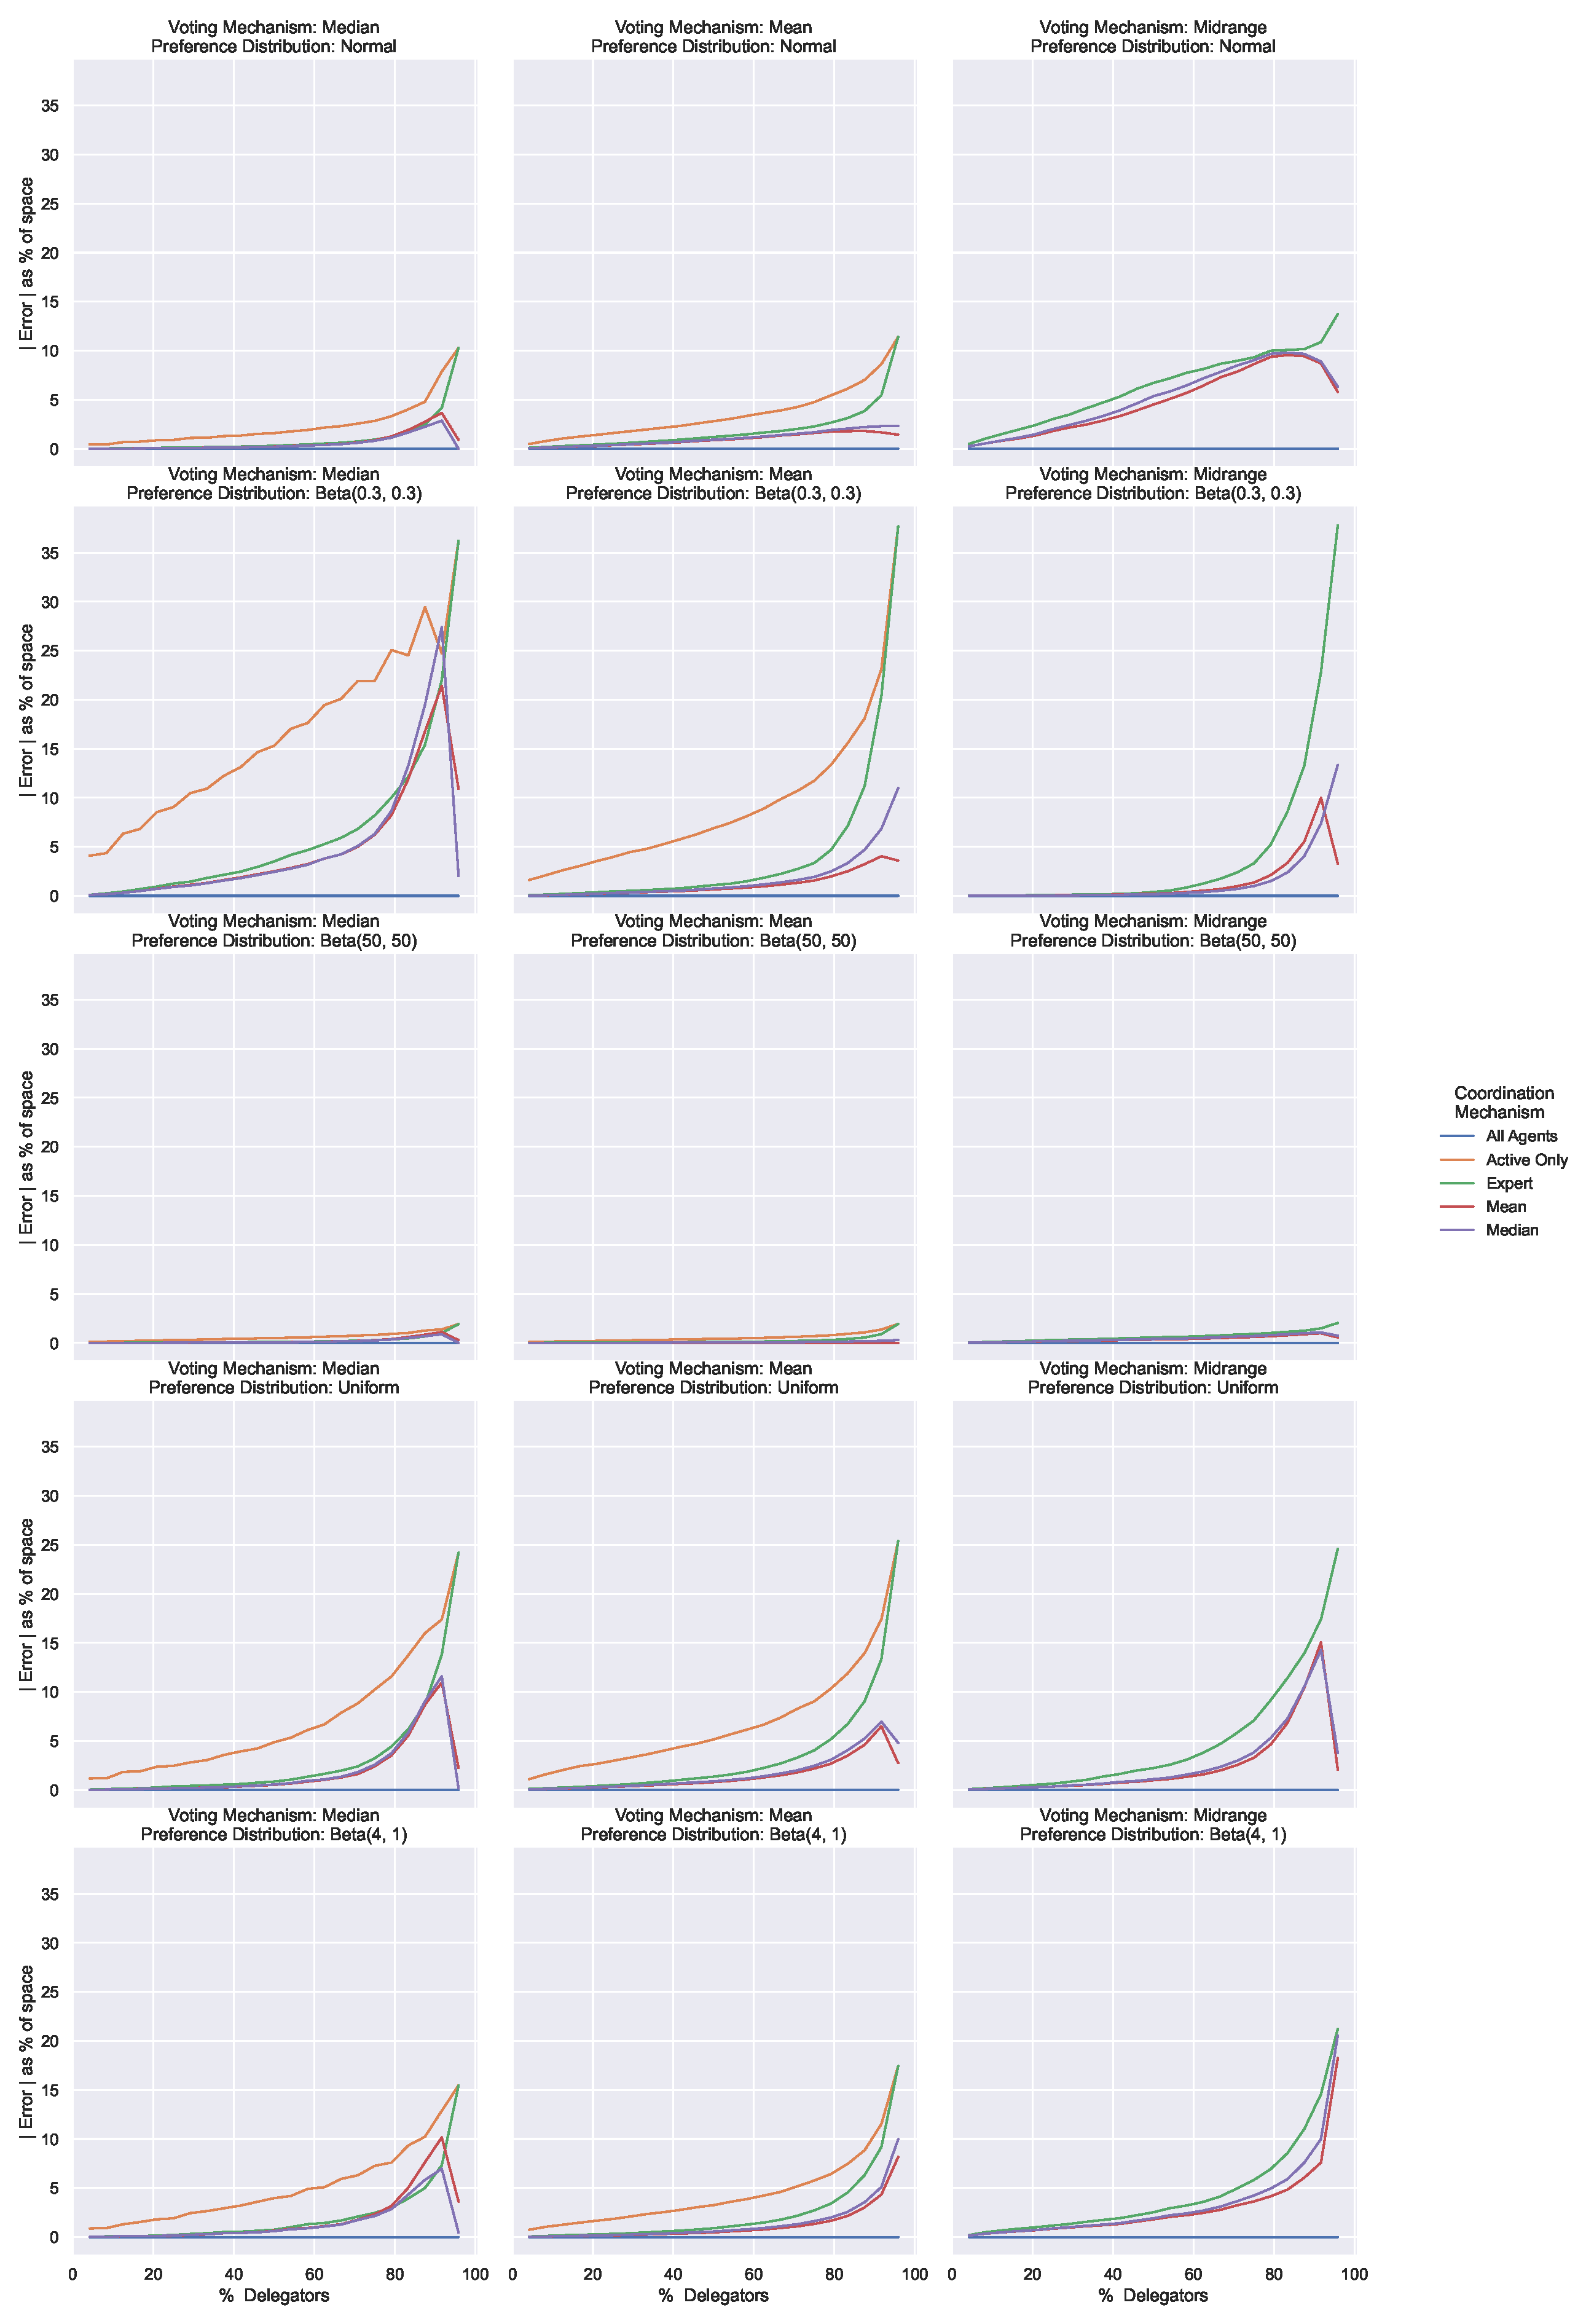
\includegraphics[scale=0.35]
    {content/chapter2/figures/distribution_error_as_percent_of_space_abs_mean}
    \caption{
        The absolute error as a percent of the preference space by coordination
        mechanism for each voting mechanism and preference distribution.
        Averaged over 1024 total runs.
        There are 24 total agents.
    }
    \label{fig:distribution-error-as-percent-of-space-abs-mean}
\end{figure}

Unsurprisingly, the tighter the probability density function (PDF) of a distribution,
the less error it has overall due to many votes being close to each other.
\betadistribution{50}{50} and \gaussian are two such distributions.
Nevertheless, these plots show the increase in error is consistent regardless of the
mechanisms or distributions used.
Mean and Median coordination mechanisms show a similar amount of error, while Expert
shows slightly more except when a large portion of the population is delegating and
when using the Midrange voting mechanism.
% \vicki{
%     I would guess you would see more problems with the median, as the median cannot
%     be accurately determined when they vote as a block.
%     If this is the case, it should be identified.
%     In general, median is considered better as it isn't manipulable.
% }
Interestingly, this seems to indicate again that it does not matter how you do proxy
voting so long as it is done.
Additionally, it should be noted the mechanisms perform well on most preference
distributions, including the asymmetrical distribution \betadistribution{4}{1}.

Unfortunately, while the error for other distributions is relatively similar,
\betadistribution{0.3}{0.3} yields considerably more error and starts accumulating
this error earlier.
\betadistribution{0.3}{0.3} represents a highly polarized topic, with its probability
density function having large spikes at either end of the preference space.
This would indicate that proxy voting, while it is still better than active-only
voting, does not work quite as well when agents have stronger, opposing opinions.  \vicki{Why does this happen?  Is it because there are so few voters?  It would seem that two strong opinions shouldn't cause more error.  This needs to be explored as two opposing opinions is a common case.}

For the median mechanism voting mechanism, this makes sense.
The median will most often be the preference of a specific agent, instead of some
value in between.
As such, the result will often be in one of the spikes in the PDF, since that is
where the majority of the agents' preferences will be, yielding higher error than when
using the Mean or Midrange voting mechanisms.

With the other voting mechanisms, the error is similar to other distributions using
the same mechanisms until the vast majority of the agents are inactive.
The increase in error is because as more agents go inactive there are fewer agents able
to serve as proxies, and so there may not be as desirable of a proxy to represent
each agent.

This finding is particularly important, as often the most polarizing topics are the
most important to individuals.
While it is still more beneficial to use proxy voting than not in these polarized
cases, agents should make an extra effort to participate in-person to ensure their
voice is heard.

\subsection{Preference Change}\label{subsec:results-shift}
\autoref{fig:abs-diff-from-preference-change-error-as-percent-of-space-abs-mean} shows
the difference in error between when proxies do have a preference change and when
they don't.
In this case, the proxies were able to shift their preferences by up to 10\% of the
total preference space, while delegators kept their original preference.
This represents the proxies changing their preference for an issue after deliberation.

Unsurprisingly, the amount of error increases as more agents become inactive.
However, the coordination mechanisms are much more tightly grouped than in other
scenarios.
We also see all coordination mechanisms actually yield worse error than active-only
voting when using the Median and Mean voting mechanisms.
This might be because delegators are selecting proxies who then shift a large amount,
leaving the delegator unsatisfied.

This potentially worse outcome highlights not only the importance of actively
participating in discussions, but also that when one needs to choose a proxy the
proxy must be someone who would act as the delegator who want them to act.

\begin{landscape}
    \begin{figure}[p]
        \centering
        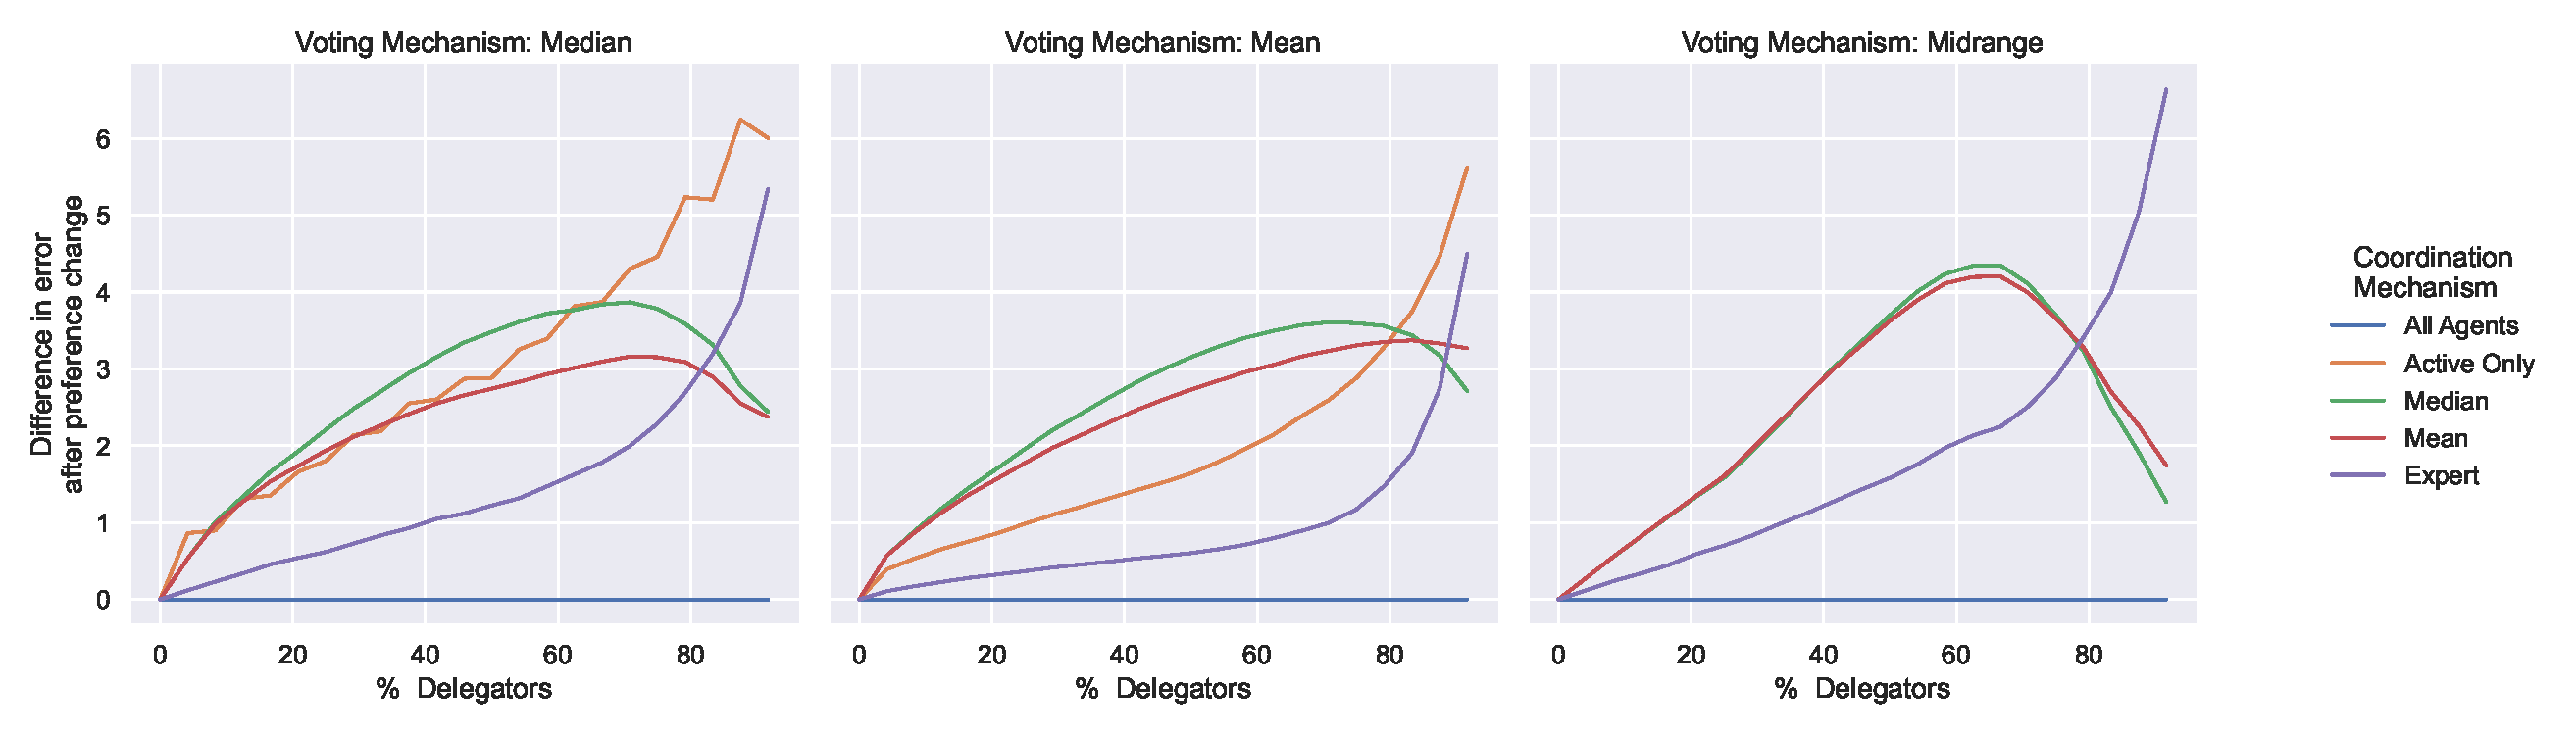
\includegraphics[scale=0.55]
        {content/chapter2/figures/abs_diff_from_preference_change_error_as_percent_of_space_abs_mean}
        \caption{
            The absolute difference in the error produced between without a
            preference change and with a preference change as a percent of space.
            Averaged over 1024 total runs.
            There are 24 total agents.
        }
        \label{fig:abs-diff-from-preference-change-error-as-percent-of-space-abs-mean}
    \end{figure}
\end{landscape}
